\documentclass[titlepage,a4paper]{article}

\usepackage{a4wide}
\usepackage[colorlinks=true,linkcolor=black,urlcolor=blue,bookmarksopen=true]{hyperref}
\usepackage{bookmark}
\usepackage{fancyhdr}
\usepackage[spanish]{babel}
\usepackage[utf8]{inputenc}
\usepackage[T1]{fontenc}
\usepackage{graphicx}
\usepackage{float}

\pagestyle{fancy} % Encabezado y pie de página
\fancyhf{}
\fancyhead[L]{TP2 - Grupo 6}
\fancyhead[R]{Algoritmos y Programación III - FIUBA}
\renewcommand{\headrulewidth}{0.4pt}
\fancyfoot[C]{\thepage}
\renewcommand{\footrulewidth}{0.4pt}

\begin{document}
\begin{titlepage} % Carátula
	\hfill
\includegraphics[width=6cm]{logofiuba.jpg}
    \centering
    \vfill
    \Huge \textbf{Trabajo Práctico 2 — Gwent}
    \vskip2cm
    \Large [75.07 / 95.02 / TB025] Algoritmos y Programación III\\
    Primer cuatrimestre de 2025 
    \vfill
    % Tabla de datos de los integrantes
    \begin{tabular}{ | l | l | l | }
      \hline
      \textbf{Nombre} & \textbf{Padrón} & \textbf{Mail} \\ \hline
      Ames Berrospi, Andy Bruno & 105366 & aames@fi.uba.ar \\ \hline
      González Lago, Mercedes & 110796 & mmgonzalez@fi.uba.ar \\ \hline
      Hirak, Jonathan Julian & 104184 & jhirak@fi.uba.ar \\ \hline
      Moore, Juan Ignacio & 112479 & jmoore@fi.uba.ar \\ \hline
      Narváez Yaguana, Gabriel Alejandro & 111432 & gnarvaez@fi.uba.ar \\ \hline
    \end{tabular}
    % Fin tabla de datos de los integrantes
    
    \vspace{1cm}
    \begin{flushleft}
    Tutor: Diego Sánchez \\
    \vspace{0.5cm}
    Nota Final: \rule{2cm}{0.4pt}
    \end{flushleft}
    \vfill
    \vfill
\end{titlepage}

\tableofcontents % Índice general
\newpage

\section{Supuestos}\label{sec:supuestos}
% Documentar todos los supuestos hechos sobre el enunciado. Asegurarse de validar con los docentes.

Ninguno de momento.

\section{Diagramas de clase}\label{sec:diagramasdeclase}
% Varios diagramas de clases, mostrando la relación estática entre las clases. Pueden agregar todo el texto necesario para aclarar y explicar su diseño de manera tal que el modelo logre comunicarse de manera efectiva.

A continuación se presenta el diagrama principal de clases del juego, que ilustra la estructura y las relaciones estáticas entre los componentes más relevantes de Gwent.

\begin{figure}[H]
    \centering
    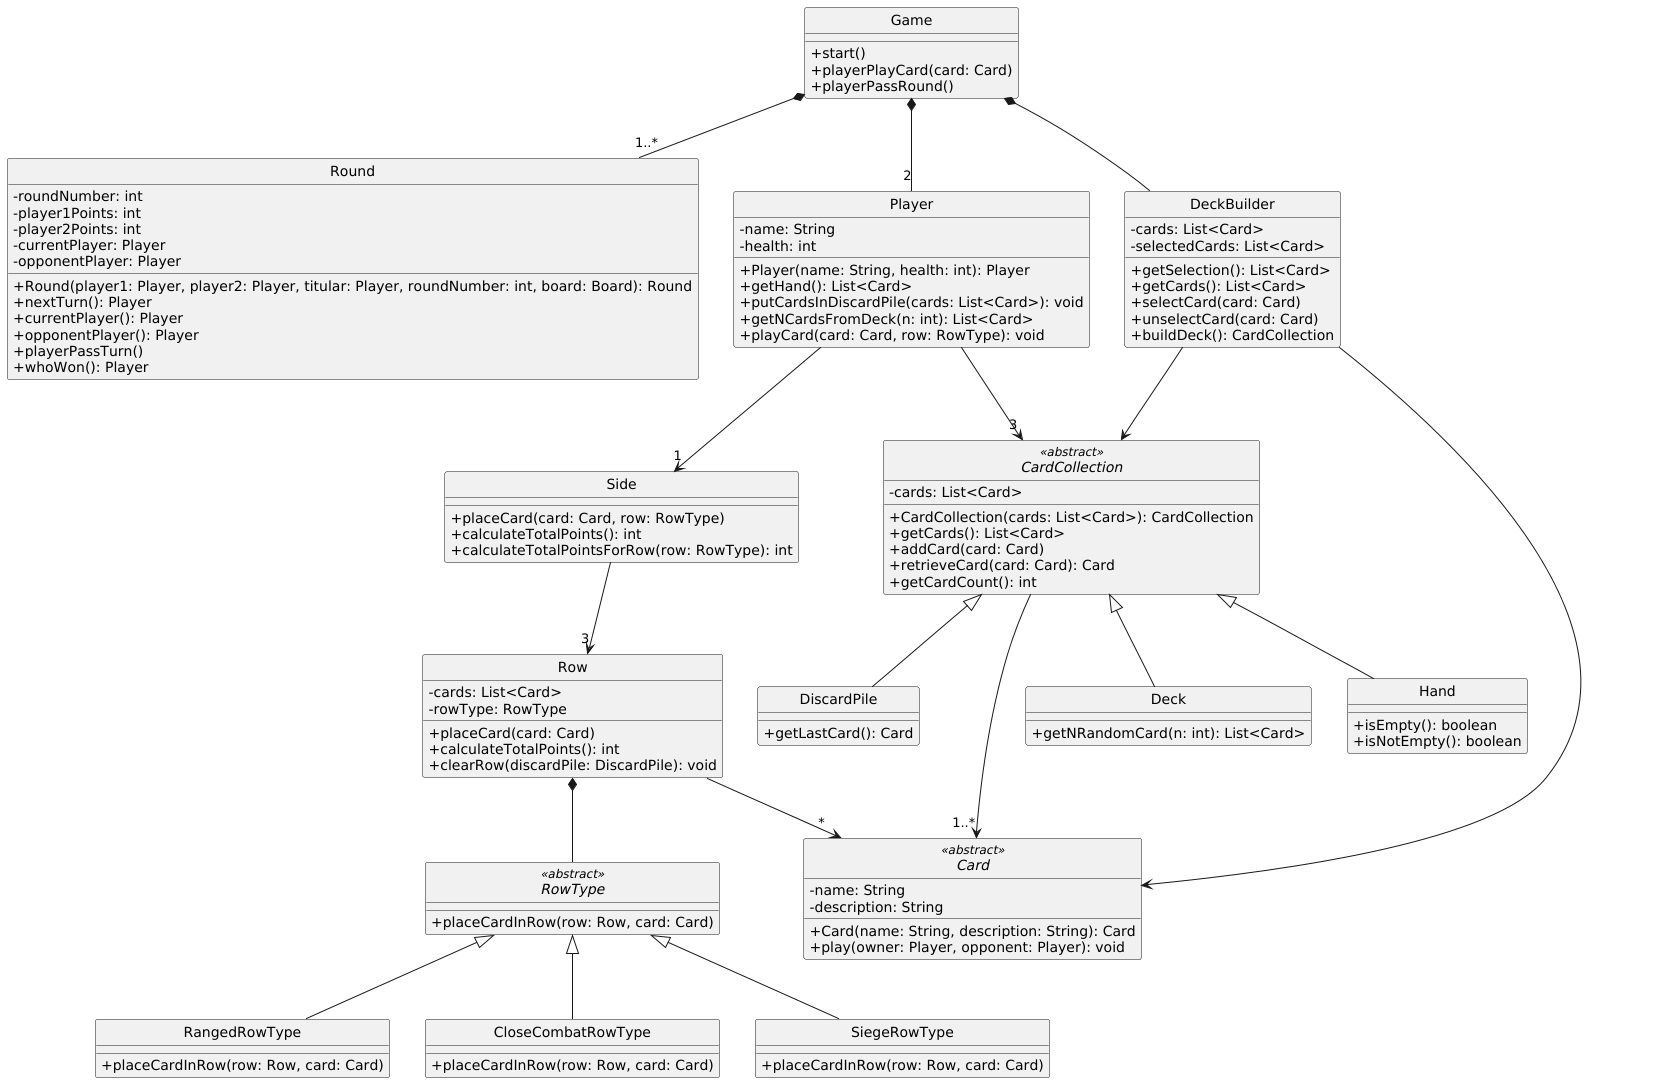
\includegraphics[width=0.95\textwidth]{../../../diagrams/classes/game.png}
    \caption{Diagrama de clases principal del juego (Game, Player, Board, Round, Deck, DeckBuilder).}
\end{figure}

\subsection*{Game}
La interacción con el conjunto de clases del juego se realiza principalmente a través de la clase \textbf{Game}, que centraliza la lógica principal y actúa como punto de entrada para las operaciones del sistema. Esta clase coordina el flujo general del juego y delega responsabilidades específicas en otras entidades clave.

\subsection*{Round}
La clase \textbf{Round} se encarga de la gestión de cada ronda y la administración de los turnos. Es responsable de determinar el siguiente jugador, identificar cuándo un jugador ha pasado (y, por lo tanto, no puede seguir jugando en esa ronda), y decidir quién resulta ganador una vez que ambos jugadores han pasado o han jugado todas sus cartas.

\subsection*{Board}

\begin{figure}[H]
    \centering
    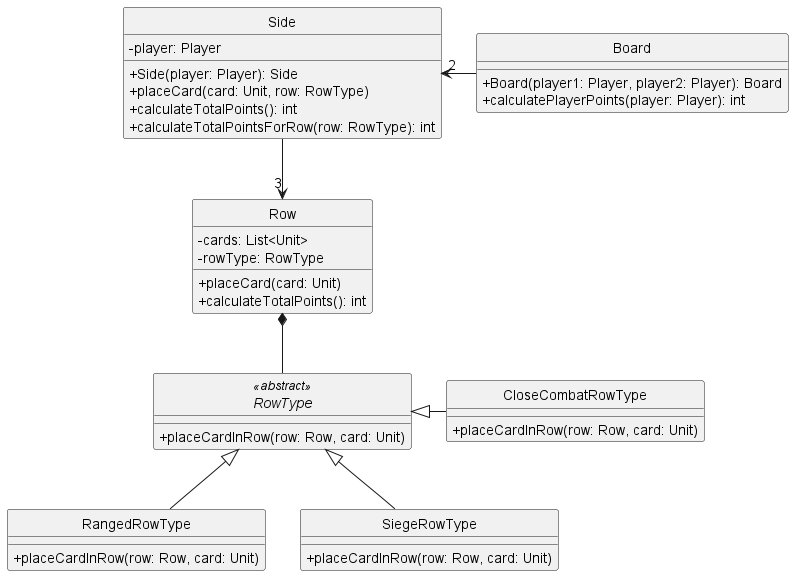
\includegraphics[width=0.7\textwidth]{../../../diagrams/classes/board.png}
    \caption{Diagrama de clases de Board, Side, Row y RowType.}
\end{figure}

La clase \textbf{Board} y sus clases asociadas (\textbf{Side} y \textbf{Row}) se ocupan del cálculo de los puntajes de las cartas jugadas y del mantenimiento del registro de las cartas presentes en el tablero. Esto permite llevar un control preciso del estado del juego y facilita la evaluación de las jugadas de cada participante.

Esta organización favorece la separación de responsabilidades y la extensibilidad del modelo, permitiendo que cada componente se enfoque en su función principal dentro del juego.

\subsection*{Player}
La clase \textbf{Player} se encarga de administrar las cartas que posee cada jugador, tanto en la mano como en el mazo y el descarte. Además, es responsable de detectar cuándo un jugador se queda sin cartas disponibles y de mantener el registro de las vidas restantes de ese jugador a lo largo de la partida.

\begin{figure}[H]
    \centering
    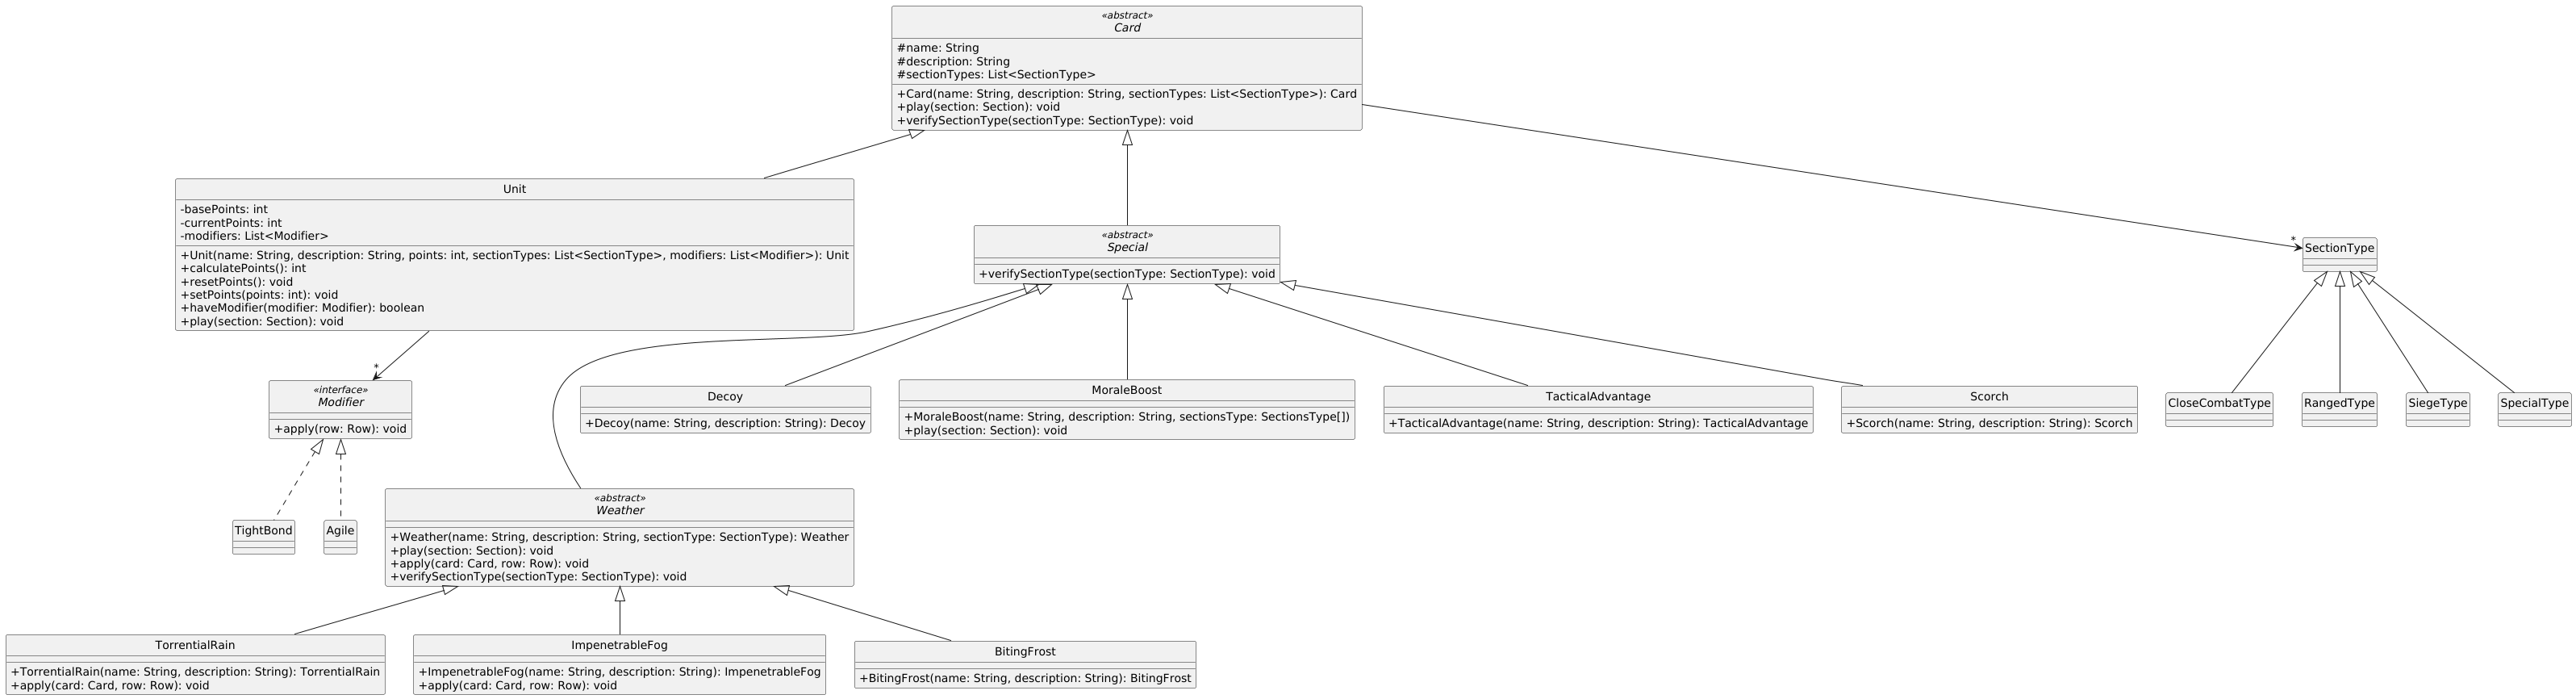
\includegraphics[width=0.7\textwidth]{../../../diagrams/classes/cards.png}
    \caption{Diagrama de clases de la jerarquía de cartas y efectos especiales.}
\end{figure}


% El diagrama más completo y detallado se encuentra en el archivo PlantUML 'boceto.plantuml' en la misma carpeta, y puede ser consultado para mayor profundidad sobre las relaciones y clases auxiliares.

\section{Diagramas de secuencia}\label{sec:diagramasdesecuencia}
% Varios diagramas de secuencia, mostrando la relación dinámica entre distintos objetos planteando una gran cantidad de escenarios que contemplen las secuencias más interesantes del modelo.


\begin{figure}[H]
    \centering
    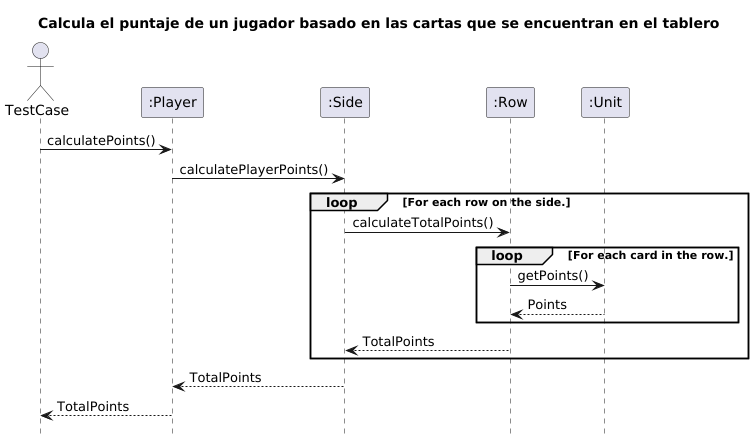
\includegraphics[width=0.8\textwidth]{../../../diagrams/sequences/DiagramaDeSecuencia1.png}
    \caption{Diagrama de secuencia de como se calcula el puntaje de un jugador.}
\end{figure}

Este diagrama refleja cómo la responsabilidad de calcular el puntaje está distribuida entre las clases Board, Side, Row y Unit, siguiendo el principio de delegación y permitiendo una estructura flexible y extensible para el manejo de las reglas de puntaje en el juego.

% \section{Diagrama de paquetes}\label{sec:diagramadepaquetes}
% Aquí irá el diagrama de paquetes UML para mostrar el acoplamiento del trabajo.

\section{Detalles de implementación}\label{sec:implementacion}
% Deben detallar/explicar qué estrategias utilizaron para resolver todos los puntos más conflictivos del trabajo práctico. Justificar el uso de herencia vs. delegación, mencionar que principio de diseño aplicaron en qué caso y mencionar qué patrones de diseño fueron utilizados y por qué motivos.

Dado que el juego consta de varias entidades con las que interactuar (jugadores, tablero, rondas, mazos, cartas, etc.), se decidió aplicar el patrón de diseño Facade. La clase principal Game actúa como fachada, centralizando la interacción con el resto de las clases y simplificando el uso del modelo para quienes utilicen el sistema. De esta manera, se oculta la complejidad interna y se facilita la extensión y el mantenimiento del código.

% \section{Excepciones}\label{sec:excepciones}
% % Explicar las excepciones creadas, con qué fin fueron creadas y cómo y dónde se las atrapa explicando qué acciones se toman al respecto una vez capturadas.

\end{document}
